% Created 2019-02-04 lun 13:41
% Intended LaTeX compiler: pdflatex
\documentclass[xcolor={usenames,svgnames,dvipsnames}]{beamer}
\usepackage[utf8]{inputenc}
\usepackage[T1]{fontenc}
\usepackage{graphicx}
\usepackage{grffile}
\usepackage{longtable}
\usepackage{wrapfig}
\usepackage{rotating}
\usepackage[normalem]{ulem}
\usepackage{amsmath}
\usepackage{textcomp}
\usepackage{amssymb}
\usepackage{capt-of}
\usepackage{hyperref}
\usepackage{color}
\usepackage{listings}
\usepackage[spanish]{babel}
\usecolortheme{rose}
\setbeamercolor{alerted text}{fg=Blue}
\setbeamerfont{alerted text}{series=\bfseries}
\setbeamerfont{block title}{series=\bfseries}
\setbeamercolor{block title}{bg=structure.fg!20!bg!50!bg}
\setbeamercolor{block body}{use=block title,bg=block title.bg}
\setbeamertemplate{navigation symbols}{}
\AtBeginSection[]{\begin{frame}[plain]\tableofcontents[currentsection,sectionstyle=show/shaded, subsectionstyle=show/hide]\end{frame}}
\AtBeginSubsection[]{\begin{frame}[plain]\tableofcontents[currentsubsection,sectionstyle=show/shaded,subsectionstyle=show/shaded/hide]\end{frame}}
\lstset{keywordstyle=\color{blue}, commentstyle=\color{gray!90}, basicstyle=\ttfamily\small, columns=fullflexible, breaklines=true,linewidth=\textwidth, backgroundcolor=\color{gray!23}, basewidth={0.5em,0.4em}, literate={¡}{{\textexclamdown}}1 {á}{{\'a}}1 {ñ}{{\~n}}1 {é}{{\'e}}1 {ó}{{\'o}}1 {í}{{\'i}}1 {ú}{{\'u}}1 {º}{{\textordmasculine}}1, showstringspaces=false}
\usepackage{mathpazo}
\hypersetup{colorlinks=true, linkcolor=Blue, urlcolor=Blue}
\usepackage{fancyvrb}
\DefineVerbatimEnvironment{verbatim}{Verbatim}{fontsize=\tiny, formatcom = {\color{black!70}}}
\beamertemplatenavigationsymbolsempty
\setbeamertemplate{footline}[frame number]
\usetheme{Goettingen}
\usefonttheme{serif}
\author{Oscar Perpiñán Lamigueiro}
\date{}
\title{Introducción al control de versiones y trabajo colaborativo con GitHub}
\hypersetup{
 pdfauthor={Oscar Perpiñán Lamigueiro},
 pdftitle={Introducción al control de versiones y trabajo colaborativo con GitHub},
 pdfkeywords={},
 pdfsubject={},
 pdfcreator={Emacs 26.1 (Org mode 9.2)}, 
 pdflang={Spanish}}
\begin{document}

\maketitle

\section{Conceptos básicos}
\label{sec:org1e990eb}
\subsection{¿Qué es el control de versiones?}
\label{sec:org0c7bcc6}

\begin{frame}[label={sec:orgfad6d7e},plain]{}
\begin{center}

\includegraphics[width=0.9\paperwidth]{figs/phdcomic_finaldoc_1.png}
\end{center}

\url{http://phdcomics.com/comics/archive.php?comicid=1531}
\end{frame}

\begin{frame}[label={sec:org3646db5},plain]{}
\begin{center}
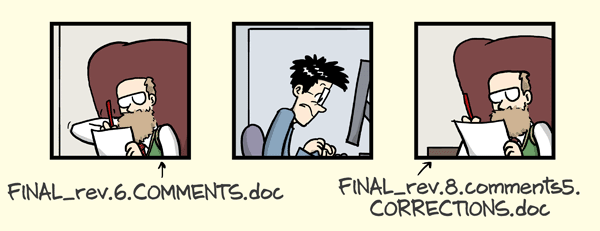
\includegraphics[width=0.9\paperwidth]{figs/phdcomic_finaldoc_2.png}
\end{center}

\url{http://phdcomics.com/comics/archive.php?comicid=1531}
\end{frame}

\begin{frame}[label={sec:org732b253},plain]{}
\begin{center}
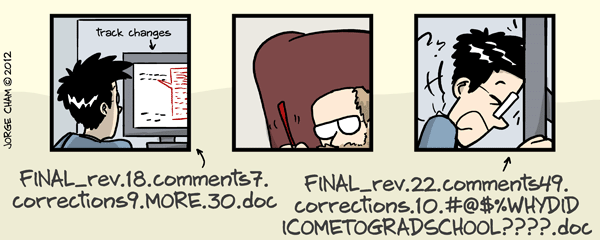
\includegraphics[width=0.9\paperwidth]{figs/phdcomic_finaldoc_3.png}
\end{center}

\url{http://phdcomics.com/comics/archive.php?comicid=1531}
\end{frame}

\begin{frame}[label={sec:org55dccbb}]{¿Qué es el control de versiones y por qué debería importarte?}
\begin{quote}
El control de versiones es un sistema que \alert{registra los cambios}
realizados sobre un archivo o conjunto de archivos a lo largo del
tiempo, de modo que se puedan \alert{recuperar} versiones específicas más
adelante.\footnote{\url{https://git-scm.com/book/es/v1/Empezando-Acerca-del-control-de-versiones}}
\end{quote}
\end{frame}

\begin{frame}[label={sec:org02109db}]{¿Qué es el control de versiones y por qué debería importarte?}
\begin{quote}
El control de versiones es el cuaderno de laboratorio en el
mundo digital. Es lo que los profesionales usan para realizar un
\alert{seguimiento} de lo que han hecho y para \alert{colaborar} con otras
personas. Cada gran proyecto de desarrollo de software se basa en
ello, y la mayoría de los programadores lo utilizan para sus
trabajos. Y \alert{no sirve sólo para software}: libros, documentos, pequeños
conjuntos de datos y cualquier cosa que cambie con el tiempo o que
deba compartirse puede y debe almacenarse en un sistema de control de
versiones.\footnote{\url{https://swcarpentry.github.io/git-novice/}}
\end{quote}
\end{frame}

\begin{frame}[label={sec:orgae83b07}]{Viajar en el tiempo}
\begin{itemize}
\item Nada que haya sido sometido a un control de versiones se pierde jamás (\emph{salvo que realmente quieras eliminarlo\ldots{}})
\item \alert{Todas} las versiones antiguas de un fichero se almacenan: un fichero se puede revertir a un estado anterior sin límites.
\end{itemize}
\end{frame}
\begin{frame}[label={sec:org3910b23}]{¿Qué? ¿Cuándo? ¿Quién?}
Un sistema de control de versiones registra:
\begin{itemize}
\item El detalle de los cambios realizados.
\item La fecha y hora en la que fueron realizados.
\item La persona que los realizó.
\end{itemize}
\end{frame}

\begin{frame}[label={sec:orgd0ac34f}]{Trabajo Colaborativo}
\begin{itemize}
\item Cuando un equipo de personas trabaja conjuntamente en un proyecto, es posible que se produzcan cambios incompatibles en un mismo fichero.
\item El sistema de control de versiones \alert{impide} cambios simultáneos en un fichero. A cambio, permite la \alert{resolución de conflictos} y los documenta.
\end{itemize}
\end{frame}

\subsection{¿Qué son Git y GitHub?}
\label{sec:org58bbeeb}

\begin{frame}[label={sec:orgaefe486},fragile]{Git es un Sistema de Control de Versiones}
 Git es una herramienta software (accesible mediante línea de comandos con \texttt{git}) que implementa un Sistema de Control de Versiones.

\begin{center}
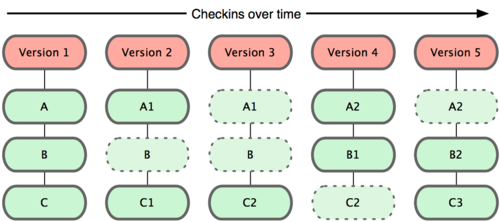
\includegraphics[width=.9\linewidth]{figs/git_model.png}
\end{center}
\end{frame}

\begin{frame}[label={sec:org27a957f}]{Git es un Sistema de Control de Versiones}
Cada vez que se ejecuta un cambio en una estructura de ficheros controlada con Git, realiza una \guillemotleft{}foto\guillemotright{} del estado de los archivos en ese momento, y guarda una referencia a esa instantánea. 
\begin{center}
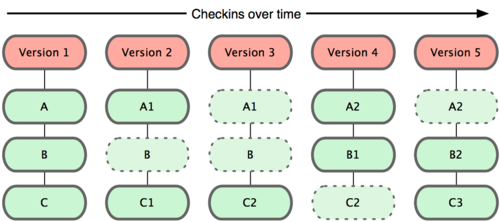
\includegraphics[width=.9\linewidth]{figs/git_model.png}
\end{center}
\end{frame}

\begin{frame}[label={sec:org7314a6a}]{Git es un Sistema de Control de Versiones}
Por eficiencia, Git no almacena los archivos sin modificaciones sino un enlace al archivo anterior idéntico que ya está almacenado

\begin{center}
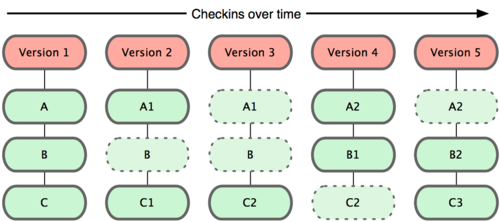
\includegraphics[width=.9\linewidth]{figs/git_model.png}
\end{center}
\end{frame}

\begin{frame}[label={sec:org74eb9c0}]{Los estados de Git}
\begin{itemize}
\item El desarrollador incorpora uno o varios ficheros al control de versiones. (\emph{tracked})
\item Realiza modificaciones en los ficheros (\emph{modified}).
\item Incorpora esos ficheros modificados al área de preparación (\emph{staged}).
\item Finalmente, confirma todos los cambios del área de preparación: se realiza la instantánea de los ficheros. (\emph{committed})
\end{itemize}
\begin{center}
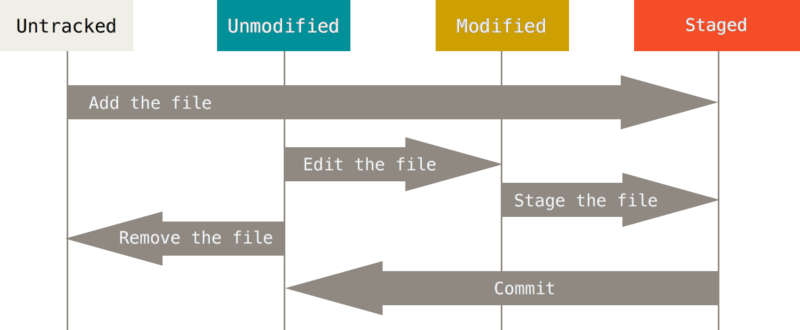
\includegraphics[height=0.4\textheight]{figs/git_estados.png}
\end{center}
\end{frame}

\begin{frame}[label={sec:org124427f},fragile]{¿Qué es GitHub?}
 \begin{itemize}
\item GitHub es la plataforma de alojamiento de código más importante a nivel mundial.
\item Emplea el sistema de control de versiones \texttt{git}
\item Ofrece una amplia variedad de funcionalidades
\begin{itemize}
\item Alojamiento de código
\item Revisión de código
\item Trabajo colaborativo
\item Publicación de páginas web
\end{itemize}
\end{itemize}
\end{frame}

\section{Uso de \texttt{git} y \texttt{GitHub}}
\label{sec:org3f35e3f}

\subsection{Primeros Pasos}
\label{sec:orga44b909}
\begin{frame}[label={sec:orgf3d2964}]{Creación de una cuenta en GitHub}
\url{https://github.com/join}

\begin{center}
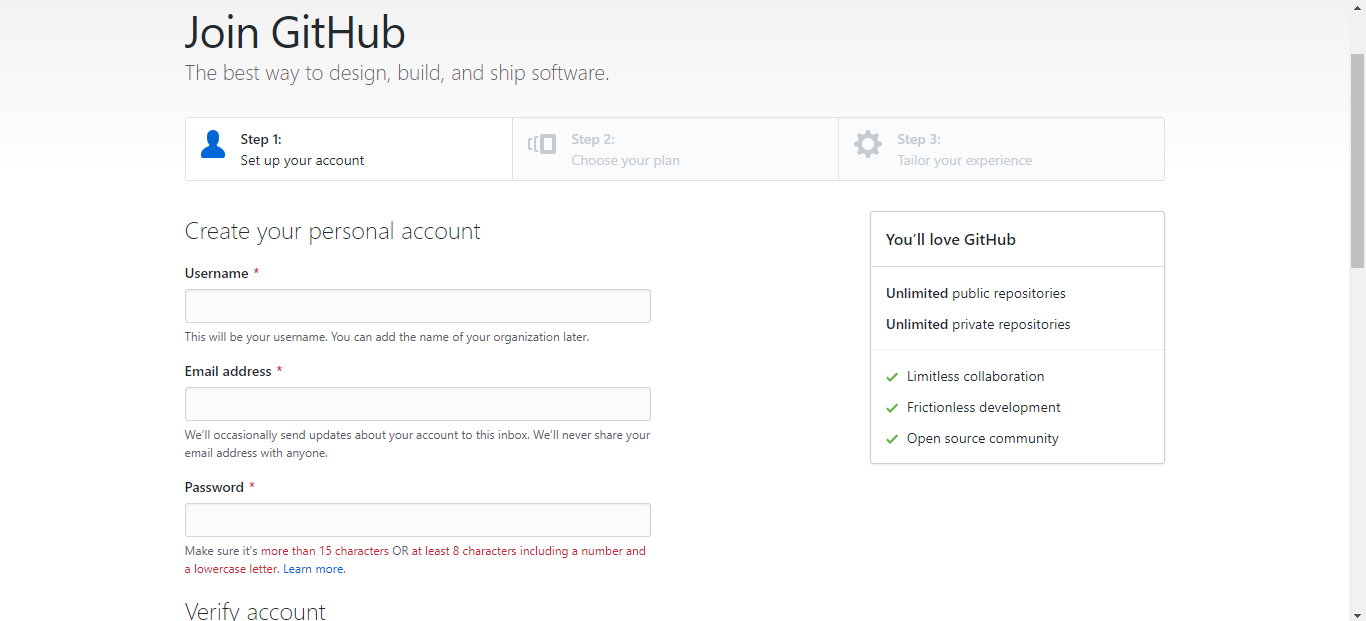
\includegraphics[width=.9\linewidth]{figs/GitHub_Join.png}
\end{center}

Más información en \href{https://help.github.com/articles/signing-up-for-a-new-github-account/}{New GitHub account}
\end{frame}

\begin{frame}[label={sec:orgefebe4e}]{Instalación de GitHub Desktop}
\url{https://desktop.github.com/}

\begin{center}

\includegraphics[width=.9\linewidth]{figs/GitHub_Desktop.png}
\end{center}
\end{frame}

\begin{frame}[label={sec:org3f8f072}]{Conectamos Git, GitHub y GitHub Desktop}
\begin{itemize}
\item Una vez instalado comienza el proceso de autenticación, usando las credenciales del paso anterior\footnote{Más información en \href{https://help.github.com/desktop/guides/getting-started-with-github-desktop/authenticating-to-github/}{Authenticating to GitHub}.}.
\end{itemize}

\begin{center}
\boxed{File > Options > Accounts > Sign\ In}
\end{center}


\begin{itemize}
\item A continuación, conectamos la información de usuario con Git\footnote{Más información en \href{https://help.github.com/desktop/guides/getting-started-with-github-desktop/configuring-git-for-github-desktop/}{Configuring Git}.}.
\end{itemize}

\begin{center}
\boxed{File > Options > Git}
\end{center}
\end{frame}


\begin{frame}[label={sec:orga6b9464}]{Nuevo repositorio desde github.com}
\url{https://github.com/new}

\begin{center}
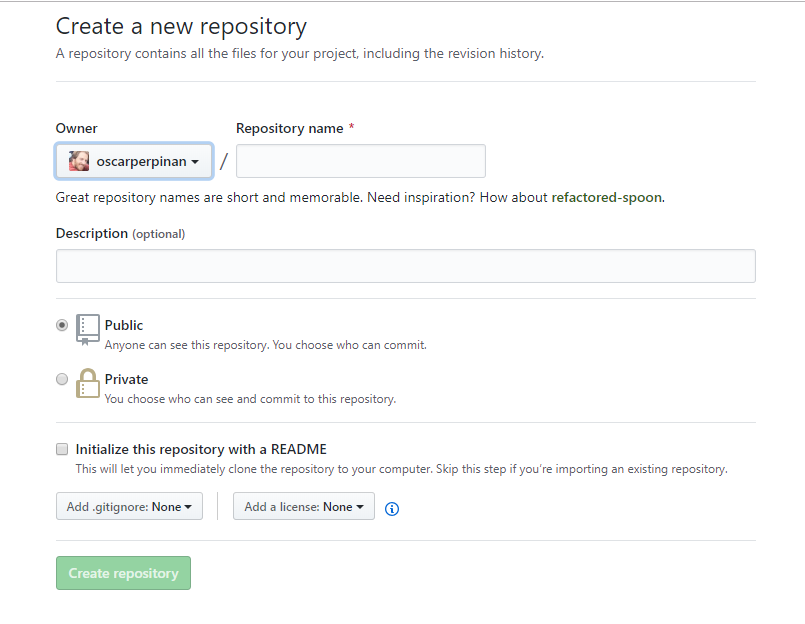
\includegraphics[width=.9\linewidth]{figs/GitHub_New_Repository.png}
\end{center}
\end{frame}

\begin{frame}[label={sec:org2de67ba}]{Nuevo repositorio desde GitHub Desktop}
\begin{center}
\boxed{File > New\ Repository}
\end{center}

\begin{center}
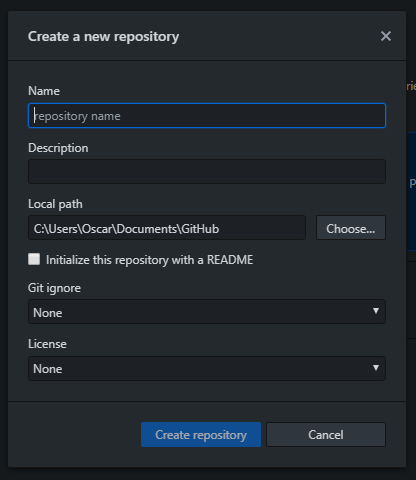
\includegraphics[height=0.8\textheight]{figs/Desktop_NewRepository.png}
\end{center}
\end{frame}

\begin{frame}[label={sec:orgb0acf29}]{Clonar un repositorio remoto}
Si hemos creado el repositorio desde github.com (\emph{repositorio remoto}), hay que clonarlo (\emph{copia local}).

\begin{center}
\boxed{File > Clone\ Repository}
\end{center}

\begin{center}
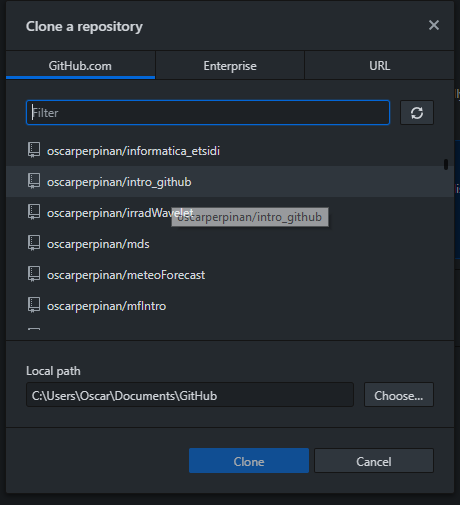
\includegraphics[height=0.7\textheight]{figs/Desktop_CloneRepository.png}
\end{center}
\end{frame}

\begin{frame}[label={sec:org1ef1b76}]{Publicar un repositorio local}
Si hemos creado el repositorio desde GitHub Desktop (\emph{repositorio local}), hay que publicarlo en github.com (\emph{remoto})

\begin{center}
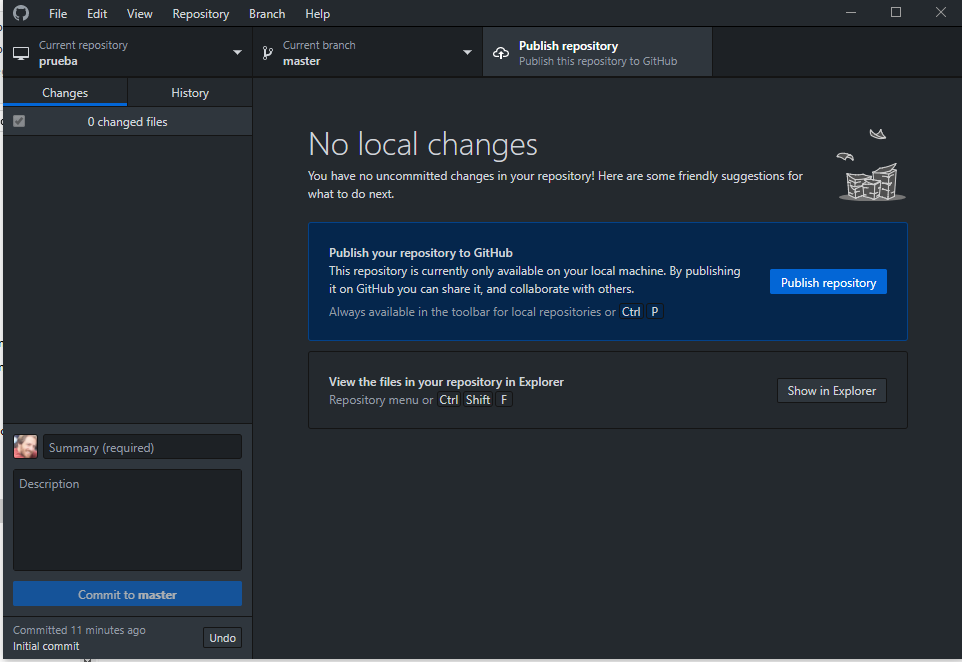
\includegraphics[width=.9\linewidth]{figs/Desktop_PublishRepository.png}
\end{center}
\end{frame}

\begin{frame}[label={sec:orga93426a},fragile]{Consejos básicos}
 \begin{itemize}
\item Elige bien el \texttt{.gitignore} (adecuado al proyecto). Veáse \url{https://github.com/github/gitignore}.
\item No olvides cumplimentar el \texttt{README.md}. Para el formato veáse \href{https://help.github.com/articles/basic-writing-and-formatting-syntax/}{Formatting syntax}.
\item Elige una licencia adecuada a tu proyecto y a tus intereses actuales y futuros. Veáse \url{https://choosealicense.com}.
\end{itemize}
\end{frame}


\subsection{Flujo de Trabajo}
\label{sec:orga6b6f34}

\begin{frame}[label={sec:org0b083c7},fragile]{Realizar y confirmar cambios (\texttt{add} y \texttt{commit})}
 \begin{columns}
\begin{column}{0.5\columnwidth}
\begin{itemize}
\item Modifica los ficheros de la copia local.
\item Añade los cambios realizados a la siguiente \guillemotleft{}instantánea\guillemotright{} del repositorio:
\end{itemize}
\begin{center}
\texttt{git add}
\end{center}
\begin{itemize}
\item Confirma los cambios (escribiendo un resumen de lo realizado):
\end{itemize}
\begin{center}
\texttt{git commit}
\end{center}
\end{column}

\begin{column}{0.5\columnwidth}
\begin{center}
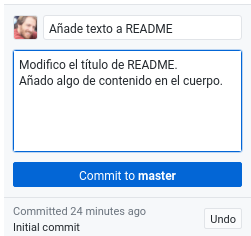
\includegraphics[width=.9\linewidth]{figs/git_commit.png}
\end{center}
\end{column}
\end{columns}
\end{frame}

\begin{frame}[label={sec:org44cbae1},fragile]{Publicar cambios (\texttt{push})}
 Para sincronizar los cambios realizados en la copia local con el repositorio remoto hay que publicar mediante \texttt{git push}.
\end{frame}
\begin{frame}[label={sec:org7f3fc6f},fragile]{Recibir cambios de un repositorio remoto}
 Para obtener los cambios recientes que existan en el repositorio y no en la copia local hay que emplear \texttt{git pull}, que es la combinación de la secuencia:
\begin{enumerate}
\item \texttt{git fetch}, obtener datos recientes del repositorio.
\item \texttt{git merge}, combinarlos con la copia local.
\end{enumerate}
\end{frame}

\section{Trabajo en colaboración}
\label{sec:org71f1610}
\subsection{Ramas (\texttt{branch})}
\label{sec:org9aa3c8b}
\subsection{Combinación de código (\texttt{pull request} y \texttt{merge})}
\label{sec:orgef97ace}
\subsection{Tareas y tableros de discusión (\texttt{issues})}
\label{sec:orgc62fa49}
\subsection{Herramientas gráficas para el análisis de un repositorio}
\label{sec:org8c7a92f}
\section{GitHub Classroom}
\label{sec:orgad19371}
\section{Publicación de páginas web en GitHub}
\label{sec:orgaadbc2e}
\end{document}